% !TeX root = ../main.tex

\chapter{相关技术}
本章将介绍安卓图形栈实现的相关技术,主要包括三个部分,第一部分介绍开源安卓项目(Android Open Source Project),主要包括安卓系统架构、Soong构建系统、Native程序运行环境bionic以及
AOSP源码树结构。第二部分主要介绍安卓图形系统结构,分别从低级别组件和高级别组件介绍图形系统所涉及的基本元素,分析实现龙芯显卡支持涉及哪些组件。
最后第三部分说明了现有龙芯GPU软件栈,依次介绍了核模块的功能与类型,MESA提供的数个核心组件,DRM框架和libdrm。

\section{AOSP}

\begin{figure}[h]
  \centering
  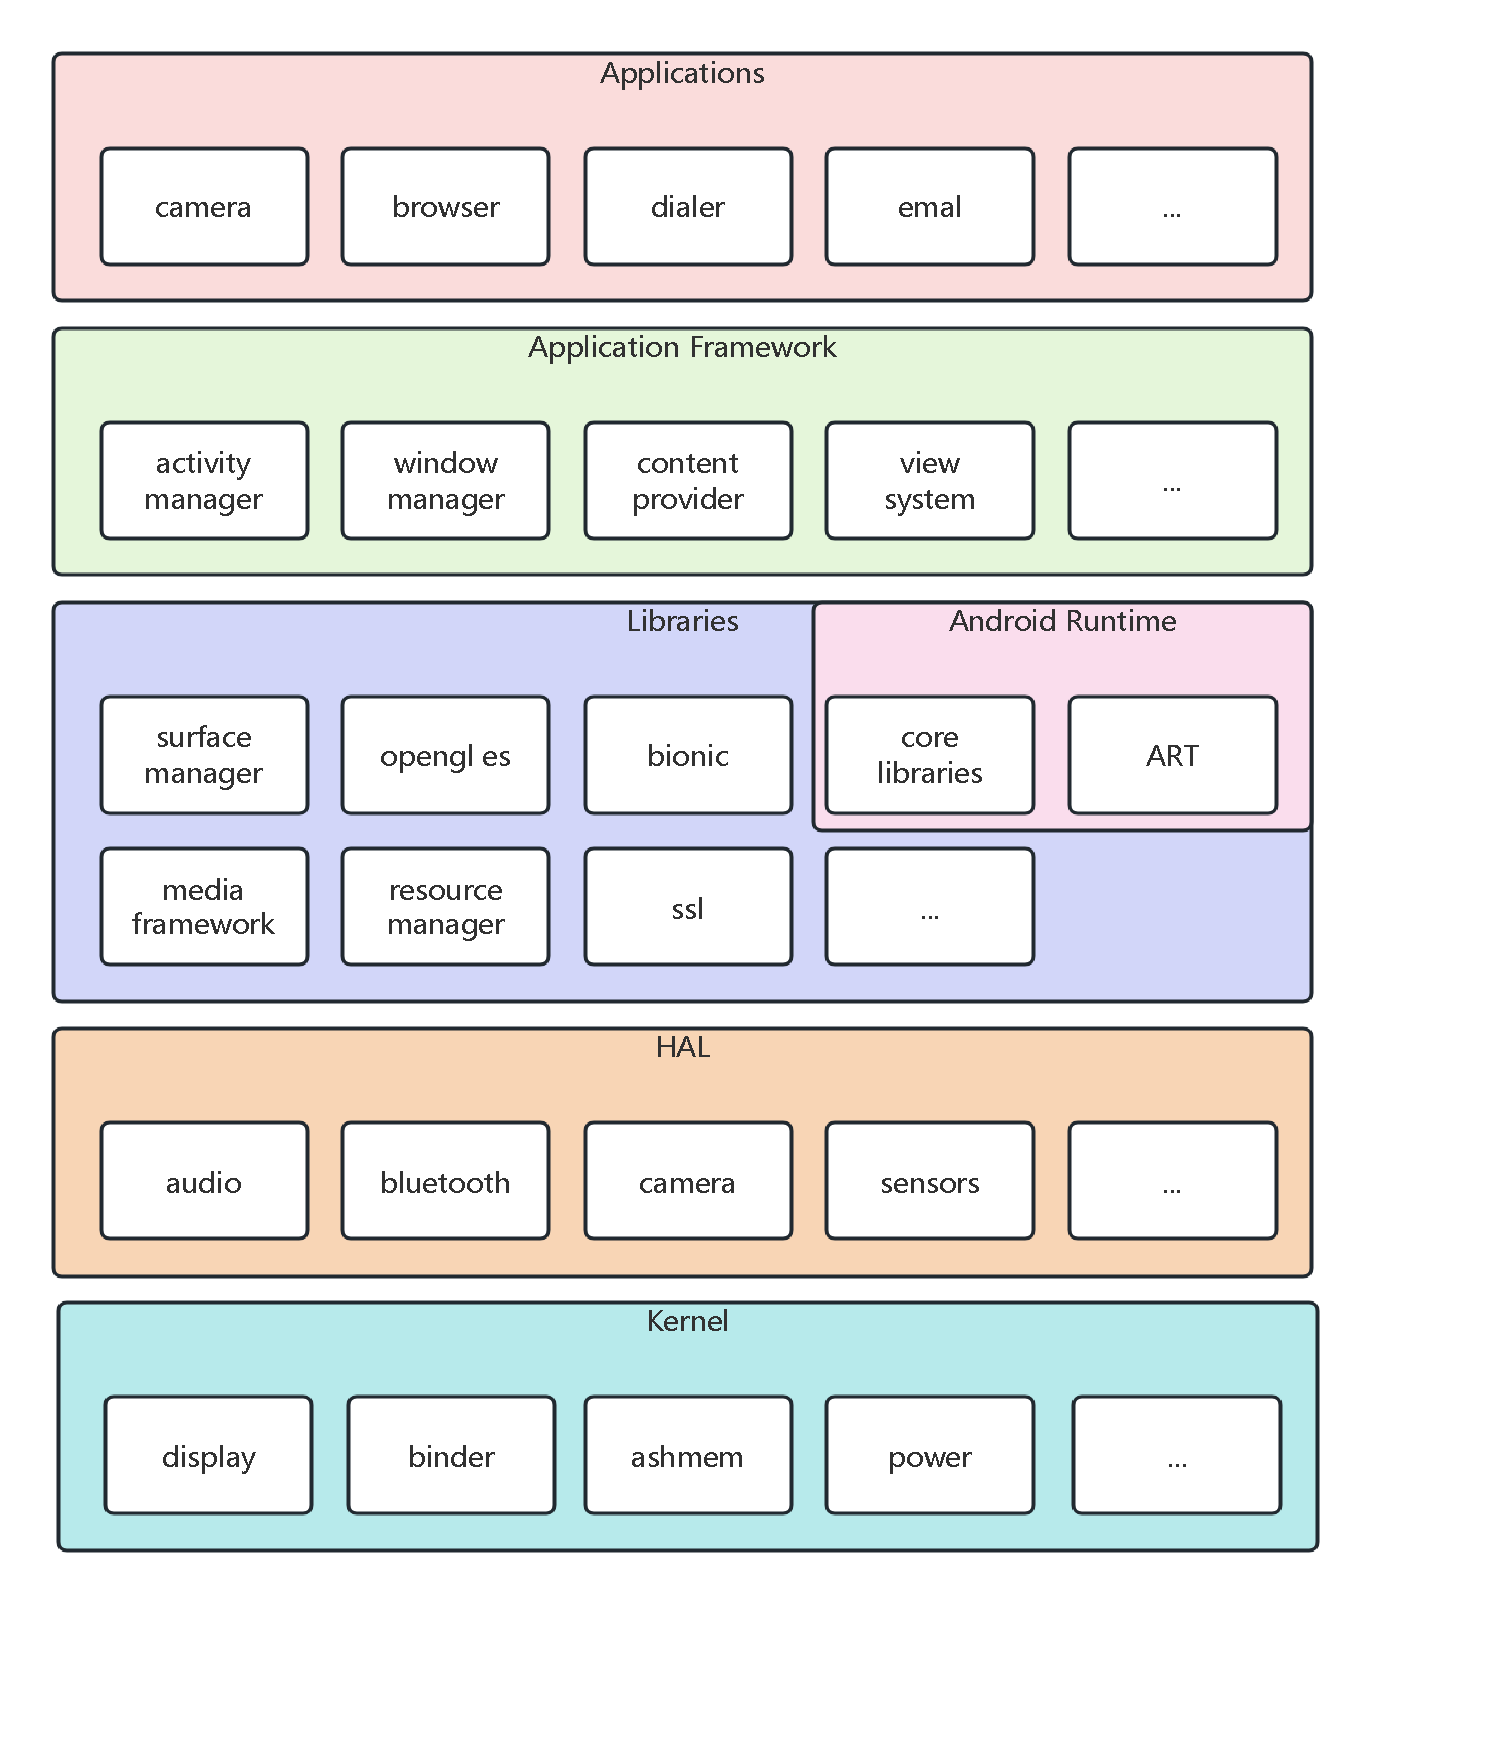
\includegraphics[width=0.8\textwidth]{安卓系统架构图.pdf}
  \caption{安卓系统架构图}
  \label{fig:安卓系统架构图}
\end{figure}

AOSP(Android Open Source Project),即安卓开源项目。
从架构上来看,Android系统的架构自下而上可以分为五个主要层次:内核层、硬件抽象层、系统运行库层(包括安卓运行时库)、应用程序框架层和应用程序层,如图\ref{fig:安卓系统架构图}。
Android 的内核基于 Linux 操作系统,Linux 内核负责系统资源的管理,如 CPU 调度、内存管理、设备管理、文件系统和网络通信等,并且包含了一些安卓特有的功能。
硬件抽象层是对底层实现的屏蔽,通过硬件逻辑和硬件接口的分离,实现上层应用对具体硬件无关的调用。
系统运行库包括核心库和 Android 运行时(ART),安卓中部分库是c/c++实现的需要这些核心库的支持,而ART 是 Android 的应用程序运行时,负责应用程序的执行,取代了旧版的 Dalvik 虚拟机。
应用程序框架层开发者提供了一个简化的 API 接口,允许他们访问系统的硬件、资源和服务,并获取所需的硬件支持。
应用程序层主要是和用户交互的应用程序,安卓提供了丰富的应用框架和工具为应用程序的多样化提供支持。

在此基础上,本课题涉及的部分包括内核层、硬件抽象层以及系统运行库层,部分包含应用程序框架层。因此,需要对AOSP整个构建系统、Native程序运行环境以及AOSP整个源码树结构进行分析,
是课题实现的基础。

\subsection{AOSP构建系统与Native程序运行环境}

\subsubsection{Soong构建系统}

\begin{figure}[h]
  \centering
  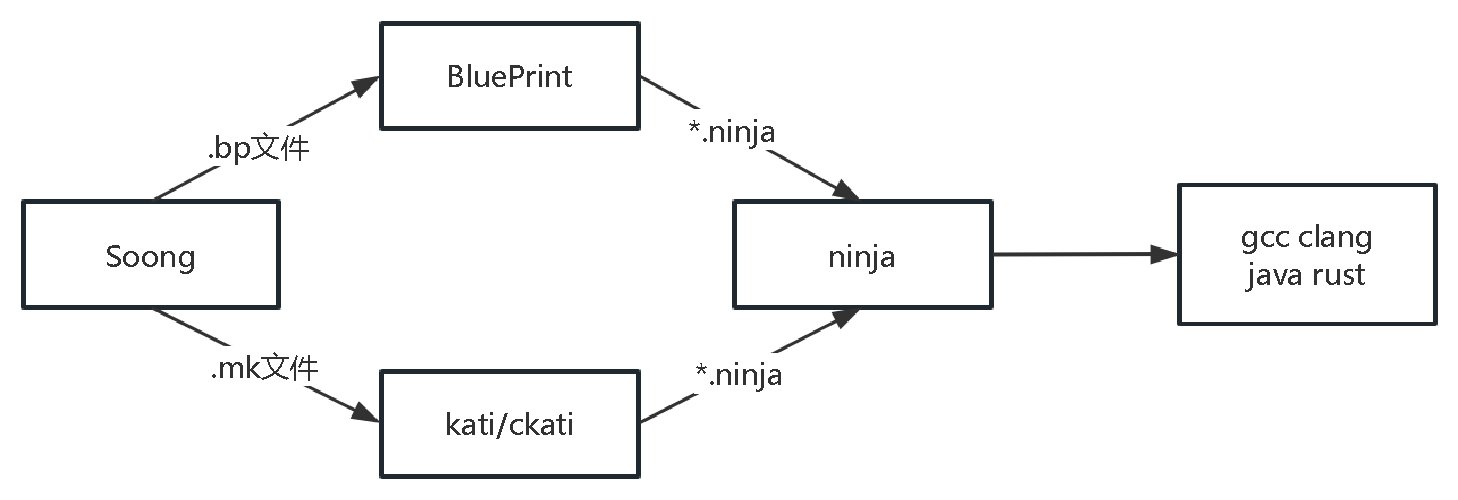
\includegraphics[width=0.8\textwidth]{soong结构示意图.pdf}
  \caption{Soong结构示意图}\label{fig:Soong结构示意图}
\end{figure}

Soong 是 Android 构建系统的一部分,主要用于替代旧的 Makefile 系统。它是一个基于 Kati GNU Make 克隆工具和Ninja构建系统组件的构建工具,旨在简化和加速 Android 的构建过程。
相较于传统的Make 编译系统,Soong支持模块化和增量构建,并且支持并行处理多个构建任务,可以加快整体构建速度。简化了配置,相较于Android.mk文件,Android.bp文件更易读,并且可以
自动管理模块之间的依赖关系,减少了手动配置的需求。

在早期的Android版本中,编译系统主要依赖于 GNU Make。这个系统使用 Makefile 文件定义构建规则,适用于较小规模的项目。由于 Android 是一个庞大的操作系统,随着功能和组件的增加,
传统的 Makefile 系统逐渐显露出其缺乏模块化以及编译时间长等缺点。Makefile 适合较简单的构建过程,但在处理复杂的依赖关系时,效率较低,且不够灵活并且随着项目的扩大,编译时间显著增加,
影响了开发效率。

而为了解决这些问题,Google 在 Android 8.0(Oreo)中引入了 Soong 作为新的构建系统。Soong 的设计旨在解决 Makefile 的诸多不足,并提供更好的性能和可维护性。
基于 Blueprint 的构建:Soong 使用了一种名为 Blueprint 的配置语言,这种语言是针对 Android 特殊需求而设计的。Blueprint 使得定义模块及其依赖关系变得更加直观和灵活。
其具有高性能、模块化和可扩展性和集成 Gradle等多种优势。Soong 通过并行化构建过程和智能依赖分析,显著提高了编译速度,使得开发者能更快地迭代。
同时支持多种模块类型,包括 Java、C/C++ 和资源文件等,适应了 Android 多样化的构建需求。开发者可以通过编写新的 Blueprint 文件来扩展 Soong 的功能。
Soong 还与 Gradle 集成,为 Android 应用的构建提供了更好的支持,使得 Android 应用开发更加灵活和便捷。结构如图\ref{fig:Soong结构示意图}

\subsubsection{bionic}

Bionic 是 Android 操作系统中的 C 标准库,实现了 POSIX 兼容的功能。它是 Android 平台的核心组件之一,具有轻量、高效等特点,
满足移动设备的特定需求,并优化性能和资源使用。Bionic 的设计考虑了 Android 的多样性和复杂性,提供基础的系统调用和库函数,
为应用程序和系统服务提供了必要的底层支持。

Bionic 的开发始于 Android 项目的早期阶段,目的是为 Android 提供一个与 GNU C 库(glibc)兼容的替代品。随着 Android 的发展,Bionic 不断演进,
以适应移动设备的需求。它的设计初衷是为了减少内存占用,提高启动速度,并提供对 Android 特有功能的支持。
主要的特性有

1.轻量级:Bionic 的核心设计理念是轻量化。它去除了许多传统 C 库中的功能,专注于满足 Android 应用的实际需求。这使得 Bionic 
在资源受限的环境中表现出色。

2.性能优化:Bionic 针对移动设备进行了多项性能优化,包括内存管理和线程处理等。其快速的启动时间和低内存占用使得 
Android 应用能够更流畅地运行。

3.POSIX 兼容性:虽然 Bionic 不是完全的 POSIX 实现,但它提供了大部分 POSIX API,这使得从其他 Unix-like 
系统移植应用变得更加容易。

4.原生开发支持:Bionic 支持 Android 的原生开发工具(NDK),允许开发者在 C 和 C++ 中编写高性能代码。
这对于需要直接与硬件交互或执行计算密集型任务的应用尤为重要。

\subsection{AOSP源码树结构介绍}
AOSP源码树的核心包含以下几个部分:

  art/: 是Android Runtime(一种App运行模式,区别于传统的Dalvik虚拟机,旨在提高Android系统的流畅性)的实现目录,包含了art库实现、dex格式转换、
  命令行工具、编译套件、测试程序等一系列组件。

  bionic/: Android的C库实现源码,是Android实现的核心组件。

  frameworks/: Android框架层核心代码的实现,是Android系统的核心部分,主要是由Java和C++编写

  system/:Android系统底层服务的实现,实现了一些核心的工具、调试工具、安全机制以及存储管理相关的功能。

  hardware/:主要是硬件抽象层的代码,包括一些旧版的HAL实现,HAL接口以及一些硬件库相关的模块。

  device/:设备厂商适配实现,主要是设备配置相关,本课题实现了LoongArch架构下的硬件配置。

  packages/:系统应用和服务的实现,包括一些核心应用程序以及第三方应用程序等,可视情况加以定制和修改

  external/:Android中使用的外部开源库。

  本文的工作集中在frameworks、device、external这几个目录下,以下几个是关键部分:

  frameworks/native/services/surfaceflinger:Android中SurfaceFlinger服务所在的源码实现,集成了CompositionEngine(合成器的客户端),
  担任图形栈生产者消费者模型中消费端的角色,用于将上层的多个源数据进行合成并输送到显示器。

  frameworks/native/libs/renderengine:Android中渲染引擎实现,包含skia引擎和gl引擎,负责系统的图形生成,该引擎的在创建时会通过获取EGL句柄、创建绑定上下文等实现对显卡驱动的调用。

  external/libdrm:图形栈中libdrm的实现,其中包含了gsgpu的实现接口以及相关测试用例

  external/mesa:图形栈中mesa的实现,mesa中包含了gallium驱动、gbm实现以及glapi等,是图形栈用户态驱动的核心库,具体会在后章节详细介绍

  external/loong-gpucomp:集成了龙芯显卡的后端实现LLVM,主要用于在mesa编译时使用。

  external/lgbm:本课题关于龙芯安卓gralloc图形内存分配器实现,根据framework框架中的gralloc4标准实现。

  external/lhwcomposer:龙芯安卓硬件混合渲染器,主要实现了合成器的服务端部分,包括设备注册与初始化以及验证与显示等功能。

  device/loongson/loongsonboard/loongson\_3a5000:龙芯3A5000硬件配置目录,包含初始化的服务顺序,部分系统属性的设置等。

  device/loongson/loongsonboard/subdevs/graphics:龙芯设备图形栈的安装配置文件,对于所需安装的产品包、产品拷贝文件、以及板卡使用的编译宏等进行配置。

\section{Android图形系统结构}\label{sec:Android图形系统结构}
Android 的图形系统是为移动设备特别设计的,结构如图\ref{fig:安卓图形子系统架构图},包含了多个组件,如 SurfaceFlinger、Hardware Composer 
和各种图形库(如 OpenGL ES 和 Vulkan)。其设计理念主要体现在以下几个方面:

深度定制:Android 的图形协议针对移动设备的资源限制和性能要求进行了优化。它通过硬件加速和资源管理,
确保在低功耗和高性能之间取得平衡。

图形合成:SurfaceFlinger 作为 Android 的图形合成器,负责将多个图形层(如应用程序窗口、系统 UI 和视频内容)
合成到一起。这种设计允许流畅的动画和用户交互,提升了用户体验。

直接硬件访问:Android 的图形协议能够直接与硬件抽象层(HAL)交互,充分利用 GPU 的性能。
这使得 Android 在图形渲染方面能够实现高效处理,尤其是在游戏和多媒体应用中。

适应性强:针对各种不同的硬件平台,Android 的图形协议能够灵活适应,支持多种显示技术和分辨率。
这种适应性使其能够在不同的设备上提供一致的用户体验。

\begin{figure}[h]
  \centering
  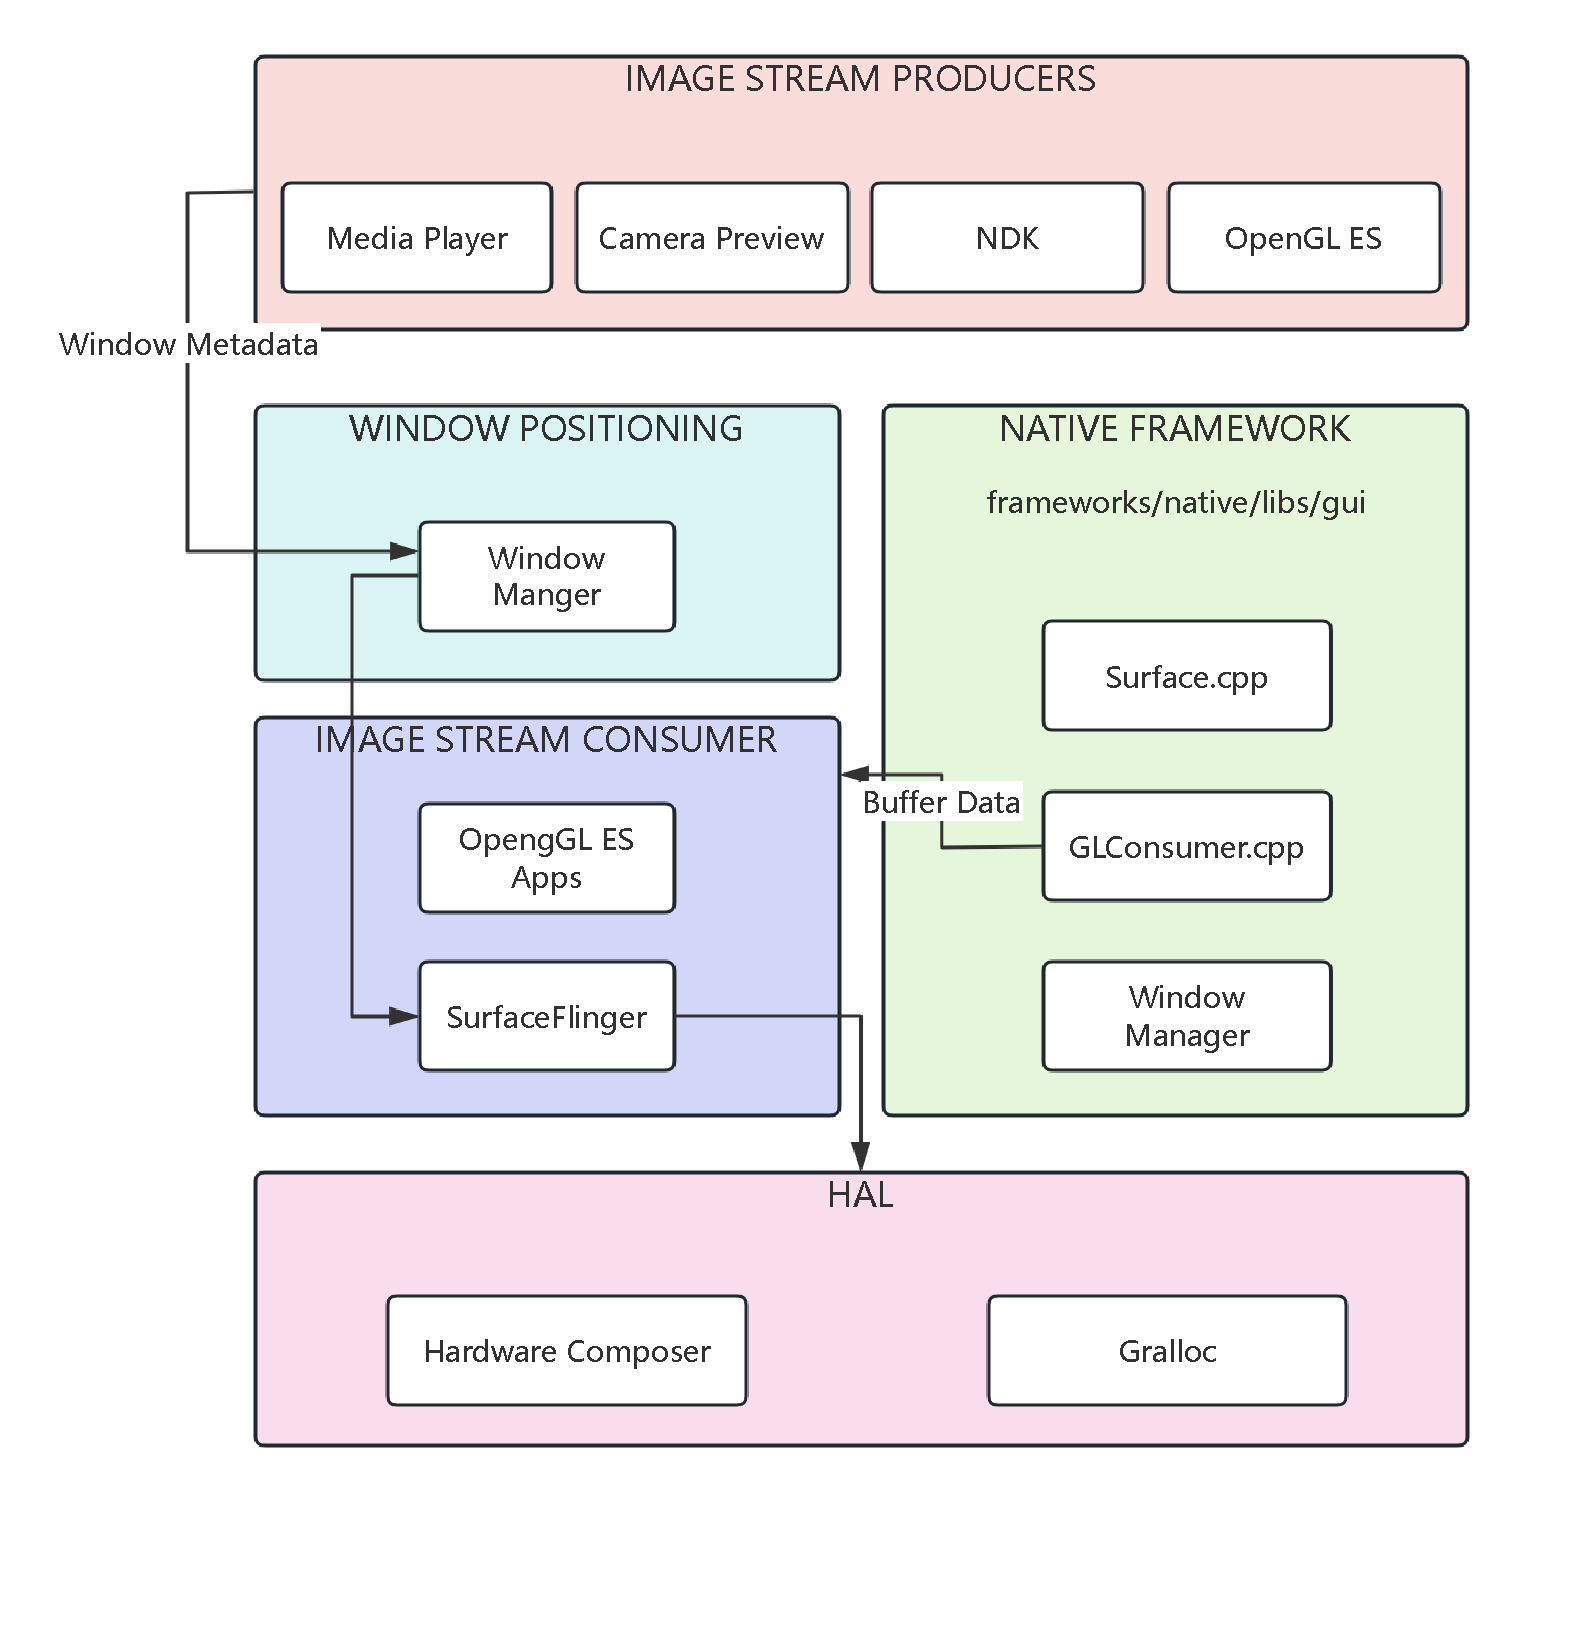
\includegraphics[width=0.8\textwidth]{安卓图形子系统架构图.pdf}
  \caption{安卓图形子系统架构图}\label{fig:安卓图形子系统架构图}
\end{figure}

以下将从低级别组件和高级别组件分别介绍Android系统级图形架构的基本元素。

\subsection{低级别组件}

\subsubsection{BufferQueue 和 gralloc}
BufferQueue 作为 Android 图形架构的核心通信机制,实现了生产者-消费者模型的高效数据流转。
该组件通过双缓冲/三缓冲策略协调图形内容生成端(如应用渲染线程)与消费端(如显示合成模块)的异步协作,有效消除帧间竞争问题。
gralloc(图形内存分配器)通过硬件抽象层接口实现跨进程图形缓冲区的生命周期管理。其核心功能包括:基于 DMA-BUF 框架的物理连续内存分配、
YUV/RGB 等像素格式的硬件对齐优化、安全上下文下的内存访问权限控制。
此分层架构使 Android 能适配不同 GPU 的异构内存架构,同时确保 SurfaceFlinger 合成效率。

\subsubsection{SurfaceFlinger和Hardware Composer}
SurfaceFlinger 作为显示合成服务,采用多层级混合合成策略:基于 HWC HAL 的硬件覆盖层合成(Overlay Composition)、
回退至 GPU 的离屏合成(Client Composition)以及元数据驱动的动态合成路径选择。
Hardware Composer 硬件抽象层通过查询机制,动态选择最优合成路径(如视频层直接送显),显著降低合成时延。

\subsubsection{图形绘制表面与软件渲染接口}
Surface 作为图形渲染的抽象画布,其实现依托于双缓冲队列的同步机制:Dequeued Buffer(应用当前写入到图形缓冲区)、Queued Buffer(等待合成的已完成缓冲区)。
Canvas API 提供基于 Skia 引擎的软件光栅化能力,是 OpenGL ES 的低级替代方案。
SurfaceHolder 通过回调接口实现 Surface 参数动态配置,其关键控制维度包括大小和格式等,为图形显示提供了灵活性。

\begin{figure}[h]
  \centering
  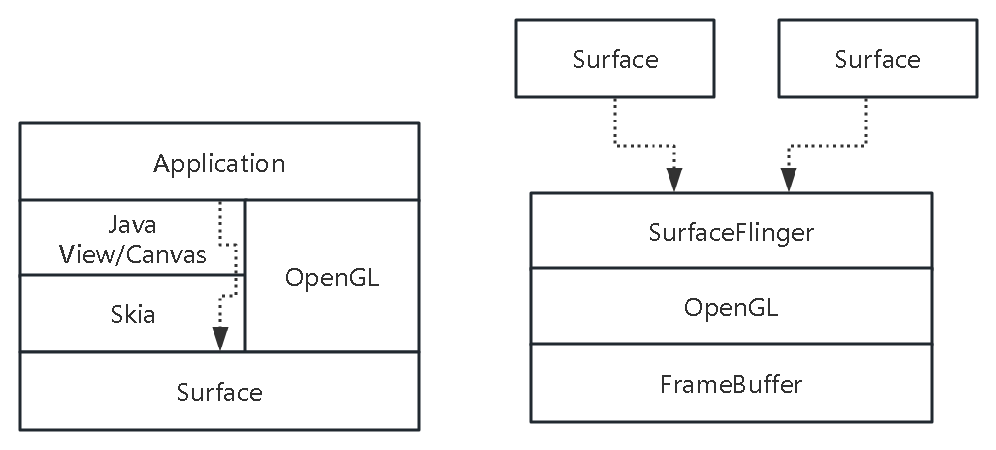
\includegraphics[width=0.8\textwidth]{Surface系统.pdf}
  \caption{Surface系统的任督二脉\cite{邓凡平2011深入理解}}\label{fig:Surface系统的任督二脉}
\end{figure}


\subsubsection{跨平台图形接口标准}
EGL(Embedded-System Graphics Library)作为 GLES 的窗口系统绑定层,实现了平台无关的渲染上下文管理、
多重缓冲交换(Double/Triple Buffering)以及图形资源生命周期同步等多种特性,确保了渲染的高效性与流畅性。
OpenGL ES (GLES) 定义了一套图形渲染 API,旨在与 EGL 结合使用。开发者可以使用 GLES 来绘制纹理多边形,
而通过 EGL 调用将渲染结果应用到屏幕上。

\subsubsection{新一代图形 API}
Vulkan\cite{sellers2016vulkan,kenwright2017getting}是一种新一代的高性能3D图形API,具有低开销和跨平台特性。与 OpenGL ES 相似,Vulkan 也提供创建高质量实时图形的工具,
但它在性能和灵活性上具备更大的优势。Vulkan 减少了 CPU 开销,使得开发者能够更直接地控制图形硬件。
此外,Vulkan 支持 SPIR-V 二进制中间语言,允许更加高效的着色器编译和执行,从而提升渲染性能和效率。

\subsection{高级别组件}

\subsubsection{SurfaceView 和 GLSurfaceView}
SurfaceView 是一种结合了 Surface 和 View 的组件。SurfaceView 的视图部分由 SurfaceFlinger 合成,
而不是由应用程序直接合成。这种设计允许在单独的线程或进程中进行渲染,使得 SurfaceView 与应用界面的渲染相互隔离,
从而提高了性能和响应性。GLSurfaceView 是 SurfaceView 的一个子类,专门用于 OpenGL ES 渲染。
它提供了管理 EGL 上下文、线程间通信以及与 Activity 生命周期交互的辅助功能,使得开发者能够更方便地进行 OpenGL ES 渲染,
尽管并不强制要求使用 GLES。

\subsubsection{SurfaceTexture}
SurfaceTexture 将 Surface 和 GLES 纹理结合在一起,创建了一个 BufferQueue。
应用程序充当这个 BufferQueue 的消费者。当生产者将新的缓冲区放入队列时,SurfaceTexture 会通知应用程序。
应用程序可以依次释放先前占用的缓冲区,从队列中获取新的缓冲区,并执行 EGL 调用,使 GLES 能够将此缓冲区作为外部纹理使用。
这种机制在 Android 7.0 中得到了增强,新增了对安全纹理视频播放的支持,允许对受保护的视频内容进行 GPU 后处理,
从而提升了视频播放的安全性和性能。

\subsubsection{TextureView}
TextureView 是一个结合了 View 和 SurfaceTexture 的组件。TextureView 封装了 SurfaceTexture,
负责处理回调以及获取新的缓冲区。在绘图时,TextureView 使用最近收到的缓冲区内容作为其数据源,
并根据 View 状态指示在需要渲染的位置和方式进行渲染。由于 View 合成始终通过 GLES 执行,
这意味着内容的更新可能导致其他 View 元素的重绘,从而确保了 UI 的一致性和动态性。

所以,若需实现对龙芯硬件的支持,主要是在低级别组件上,需要实现gralloc接口,负责图形缓冲区的分配与共享、支持不同格式的像素布局、与 GPU 显存的映射等。
同时需要实现hwcomposer的接口,完成图层合成的硬件加速,显示时序控制等功能,并保证SurfaceFLinger能够正确调用HWC和gralloc。
在图形编程接口上,而由于现有的硬件实现仅有OpenGL和OpenGL ES,暂不对vulkan作支持,需要通过通过科纳斯标准 API暴露GPU 功能,确保SurfaceFlinger的渲染引擎 Skia后端支持龙芯GPU,
这些具体支持实现将在后续章节中介绍。

% \section{安卓图形编程接口}
% 在 Android 上,图形编程接口(Graphics API)提供了与硬件图形加速进行交互的方式。
% Android 提供了多个图形编程接口,允许开发者在设备上执行各种图形和渲染任务,如用户界面渲染、游戏图形渲染、视频解码和图像处理。
% 目前常见的图形编程接口有OpenGL ES、Vulkan、OpenCL等。
% OpenGL ES 是一个用于嵌入式设备(如智能手机、平板、嵌入式设备等)的图形渲染 API,它是 OpenGL 的简化版。OpenGL ES 主要用于 2D 和 3D 图形渲染,在 Android 上被广泛使用。
% 在 Android 中,应用程序通过 GLSurfaceView(一个用于渲染 OpenGL 内容的视图)或 EGL(EGL 用于创建 OpenGL 上下文和管理图形缓冲区)来与 OpenGL ES 进行交互。
% Vulkan 是一种现代的低开销、高性能的图形和计算 API,它提供了对硬件的直接控制,相比 OpenGL ES,它提供了更细粒度的控制、更高的性能以及更低的 CPU 和 GPU 开销。
% 在 Android 上,Vulkan 需要设备支持,并且开发者需要通过 Vulkan API 来进行图形和计算任务。与 OpenGL ES 相比,Vulkan 的编程模型更复杂,但它提供了更高的性能和更灵活的图形管线。
% OpenCL 是一个开源的框架,主要用于并行计算。它允许开发者在 CPU、GPU 和其他处理器上执行计算任务,广泛用于图形计算之外的任务,如图像处理、机器学习和科学计算。
% 虽然 OpenCL 在 Android 中的使用较少,但它在需要大量计算任务的图形应用和其他计算密集型应用中仍然非常有用。
% Canvas 是 Android 中用于 2D 图形渲染的高级 API。它封装了对 OpenGL 的调用,提供了一组简单的接口,用于绘制文本、图形、位图等。Canvas 主要用于应用程序的用户界面(UI)绘制。
% Skia 是 Android 中的 2D 图形库,负责图形渲染操作,尤其是为用户界面提供支持。Skia 库支持 2D 图形、文本渲染、图像缩放、透明度和颜色操作等功能。
% SurfaceFlinger 是 Android 的图形合成器,负责将应用程序的图层(如活动窗口、动画等)组合成最终的显示图像。SurfaceFlinger 是 Android 图形架构中的一个核心组件,
% 它使用 GPU 来加速图形合成。

\section{GPU软件栈}
\subsection{核模块}
核模块 是一种内核功能扩展机制,允许将某些功能以模块的形式动态加载到操作系统的内核中。它的设计目的是增强内核的灵活性和可扩展性,使得内核在不需要重新编译或重启的情况下能够扩展和更新。
模块通过特定的接口与内核进行交互,可以动态地扩展内核的功能,而无需重新启动系统。通过内核的模块化设计,可以根据需求加载、卸载、更新不同的功能模块。
核模块的优点有:动态加载和卸载,模块不需要在系统启动时加载,而是在需要时按需加载,并可以在不需要时卸载,同时可以减少内存占用,增强了灵活性,不影响其他部分的功能。

没有模块的话,就必须得把所有实现新功能的函数都编译到内核,这种内核也叫单内核(monolithic kernels)。
单内核是一种将所有内核功能编译为一个统一的内核映像的方式,其中包括设备驱动、文件系统、网络协议栈等所有内核组件。
由于所有的功能都被编译到内核中,因此,任何功能的增加或修改都需要重新编译内核并重启操作系统。

内核模块可以根据功能的不同分为多个类型,最常见的类型包括:设备驱动模块、文件系统模块、网络协议模块、内存管理模块、安全和监控模块。
设备驱动是最常见的内核模块之一,允许操作系统通过内核访问和控制硬件设备。
文件系统模块允许内核支持不同类型的文件系统,如NTFS、ext4、FAT等。
网络协议模块用于实现网络协议栈的一部分,支持不同的网络协议(如 TCP/IP、UDP 等)。
内存管理模块用于管理系统的内存分配和回收。
而安全和监控模块用于系统安全、身份验证、访问控制和资源监控的功能模块

\subsection{MESA}
mesa\cite{mesa}是由Brian Paul于1993年8月发起的一个开源图形API软件实现,提供了一整套图形库和驱动程序,允许开发者使用标准的图形 API(如OpenGL,OpenGL ES,Vulkan等)
来进行图形渲染,而无需直接依赖硬件制造商的专有驱动程序,现由freedesktop维护并被广泛采用。
由于其本身的设计初衷就是为了提供硬件无关的图形渲染能力,所以mesa是一个跨平台跨操作系统的图形库,
可以为多个硬件平台提供支持,包括intel、amd、Nvidia等驱动均在mesa上有相关的开源实现,操作系统上支持Android、Linux、BSD 系统等。
其中有多个核心组件:

\subsubsection{驱动框架}
Mesa DRI驱动可以分为两部分,一部分是经典驱动(不基于Gallium3D 框架),另一部分是新的Gallium驱动。
经典的Mesa驱动是紧耦合的,这意味着要在现有驱动基础上实现一个其它的API规范几乎要重写这个驱动,而Gallium3D实现一套暴露现代GPU的硬件功能的API,将依赖潜在操作系统的部分分隔开来,
使得可以支持各种操作系统。如图\ref{fig:mesa驱动结构图}。在经典结构中,应用程序(APP)通过 DRI驱动程序与图形硬件进行交互,DRI 驱动程序直接管理硬件,并通过 DRM与与显示硬件进行通信。
而在Gallium 3D 结构中,有State Tracker是mesa核心和Gallium3D的接口,负责将MESA状态(混合模式,纹理状态等)和绘制命令(例如Gldrawarrays和gldrawpixels)转换为管道对象和操作
而HW driver是GPU硬件的驱动,负责将上层的状态、纹理等翻译成GPU硬件可以识别的信息,而Winsys提供了与内核交互的接口,准确来说也是使用libdrm的接口,实现对操作系统的支持。

\begin{figure}[h]
  \centering
  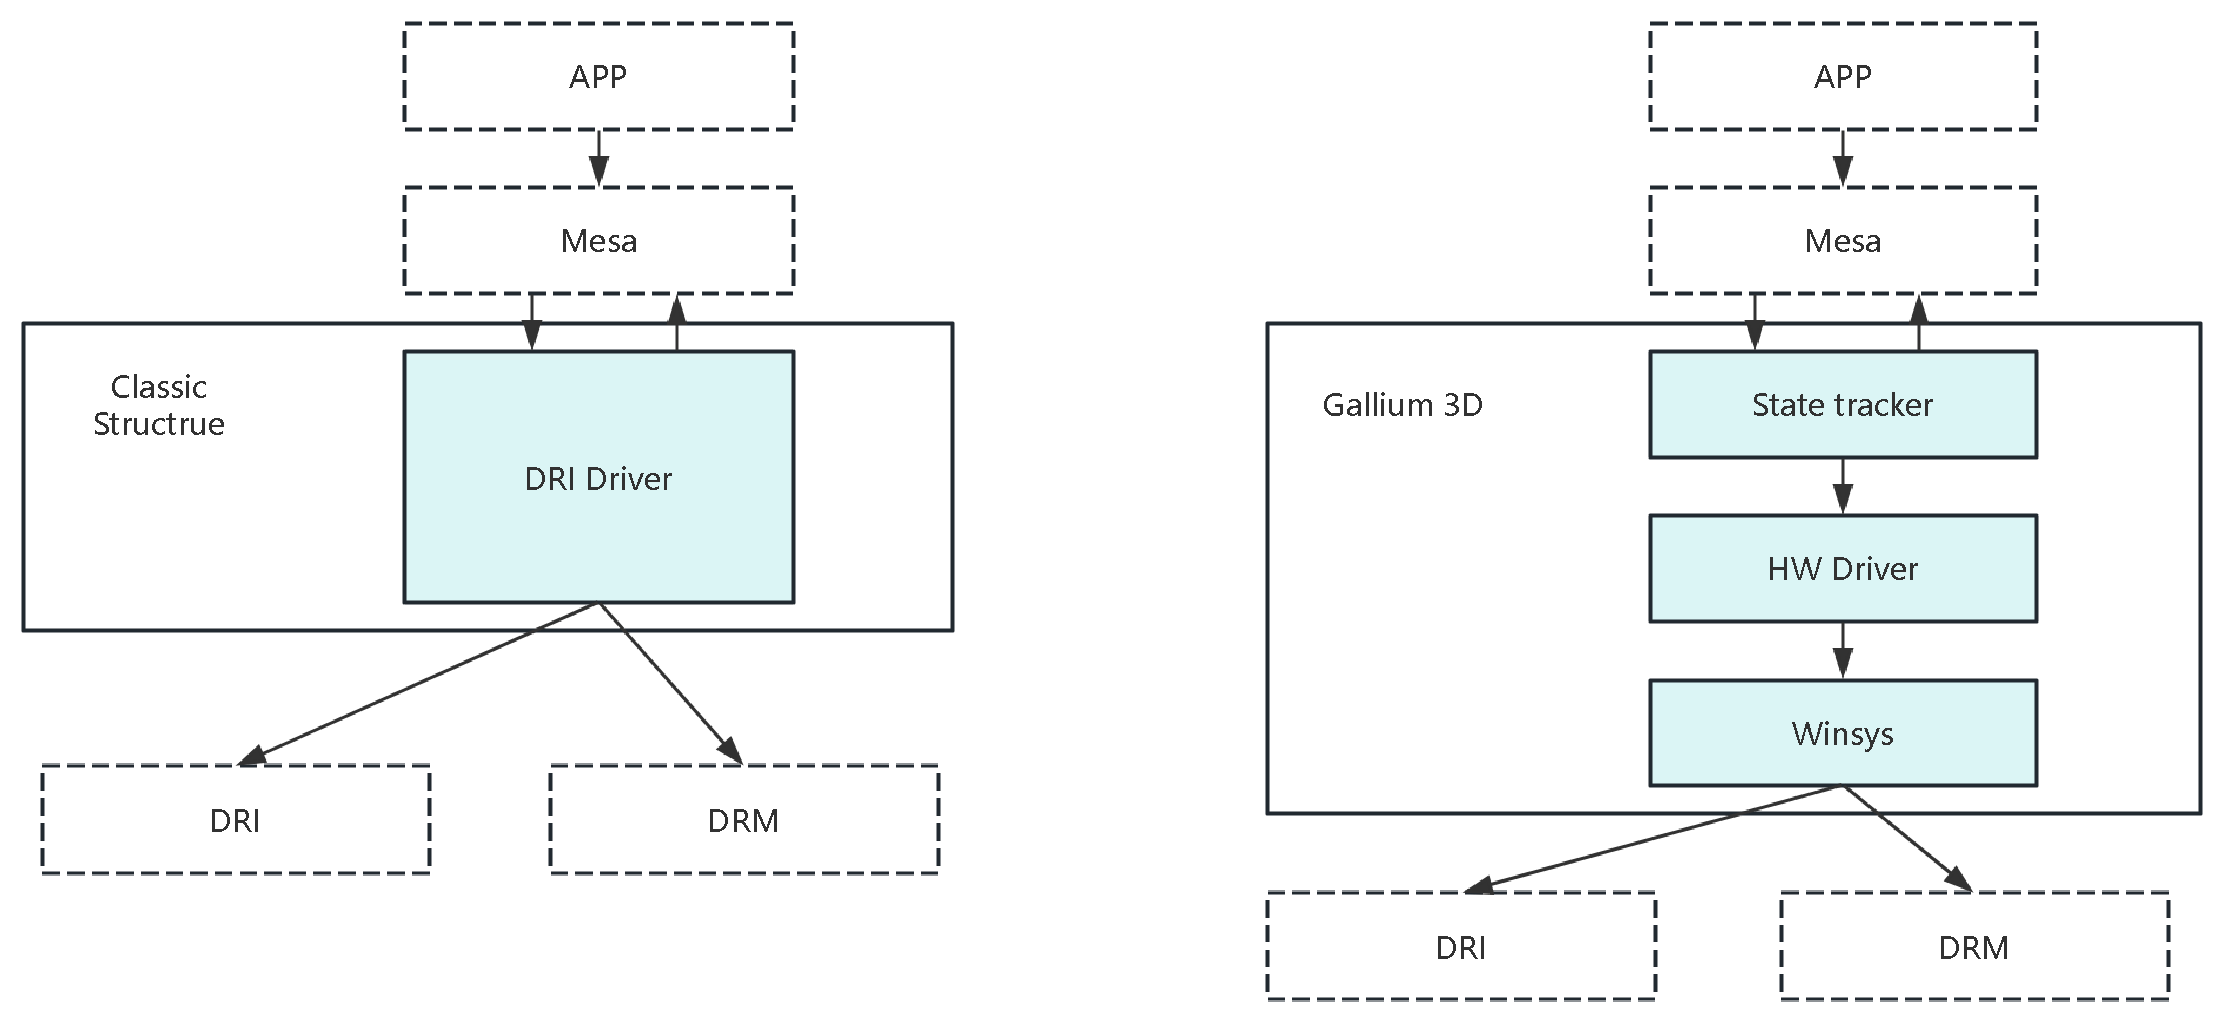
\includegraphics[width=0.8\textwidth]{mesa驱动结构图.pdf}
  \caption{mesa驱动结构图}\label{fig:mesa驱动结构图}
\end{figure}

\subsubsection{OpenGL ES}
OpenGL ES(Open Graphics Library for Embedded Systems)是一个为嵌入式系统设计的图形渲染接口,它为嵌入式设备提供了一个高效的图形渲染平台,
使其能够以较低的功耗和硬件资源要求进行复杂的图形处理。OpenGL ES 是 OpenGL\cite{2005Interpretive}一个用于桌面图形渲染的开源标准)的子集,
专为移动设备、嵌入式设备、游戏主机、电视和汽车等环境优化。
OpenGL ES 的目标是为设备提供一种跨平台的解决方案,允许开发者利用硬件加速的图形渲染,同时又不需要复杂的硬件支持。
OpengGL ES版本从1.0到3.x处于不断发展过程中,其与OpengGL的发展不完全相同,但是作为OpenGL规范的子集,两者之间版本有着大致的对应关系。

1. OpengGL ES 1.0和 OpenGL ES 1.1分别从OpenGL 1.3和OpenGL 1.5规范衍生而来,两者功能十分接近,都基于固定功能管线,所以渲染过程是由OpenGL 和 OpenGL ES 的固定功能模块
控制,而不需要开发者编写着色器程序。

2.OpengGL ES 2.0基于OpenGL 2.0的规范,采用可编程渲染管线,去除了对1.0固定功能管线的支持,依赖开发者编写着色器程序来控制渲染管线。并且相比OpenGL 2.0,
OpengGL ES 2.0去除了一些不常用的功能,专注于嵌入式设备的需求。

3.OpenGL ES 3.0 是对 OpenGL 2.x 的一次重大提升,其在功能上继承了OpenGL 3.x 的一些特性,如基于着色器的可编程渲染管线、支持多个渲染目标(MRT)、帧缓冲对象(FBO)等,然而
剔除了一些高端桌面图形功能,保持对嵌入式设备的优化。

4.OpenGL ES 3.x 其在功能上借鉴了OpenGL 4.x 规范的一些高级特性,优化了计算着色器、增强的纹理压缩、多线程支持、双缓存渲染等特性,以适应嵌入式硬件的需求。

\begin{figure}[h]
  \centering
  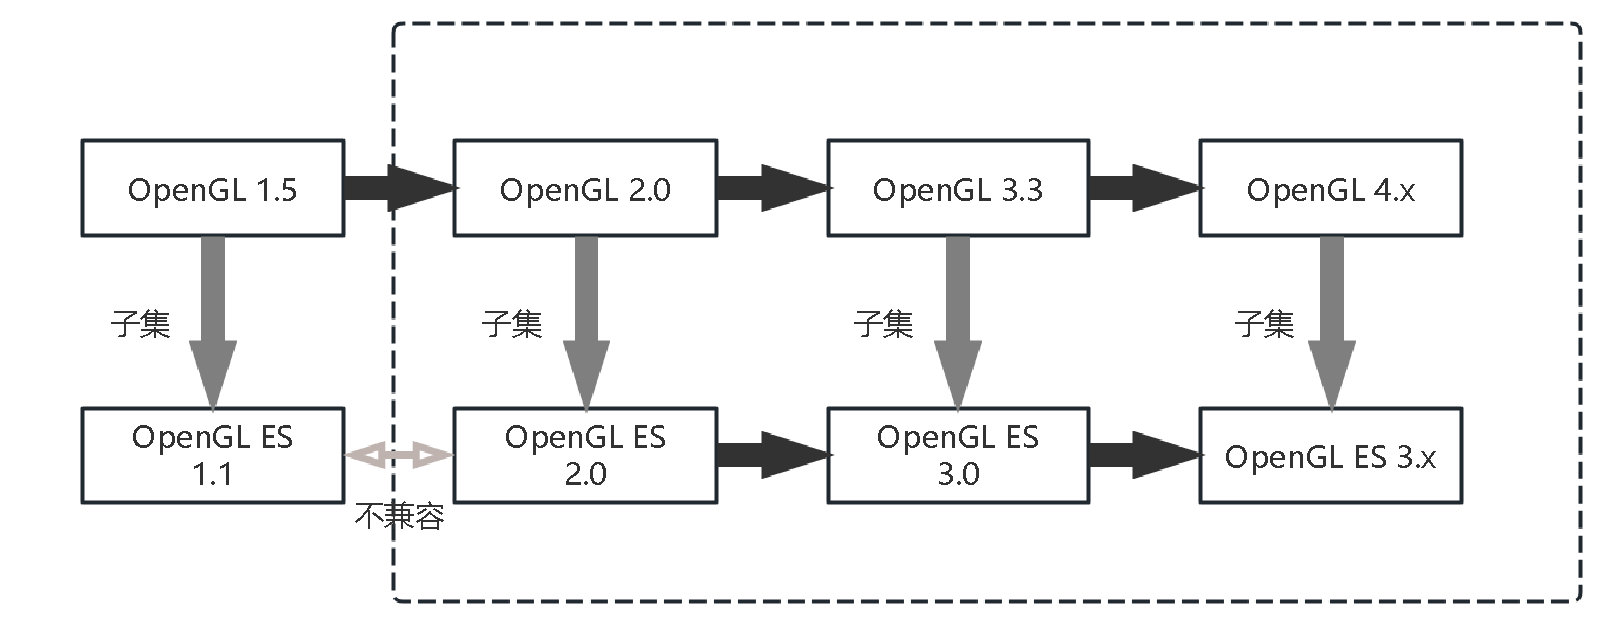
\includegraphics[width=0.8\textwidth]{OpengGL+ES版本演进.pdf}
  \caption{OpengGL ES版本演进}\label{fig:OpengGL ES版本演进}
\end{figure}

\subsubsection{GBM(Generic Buffer Manager)}
GBM是 Mesa 提供的一个内存管理库,它允许图形应用程序高效地创建、管理和共享显存缓冲区(通常是帧缓冲区)。
在图形渲染中,帧缓冲区是存储图像数据的内存区域,通常用于保存渲染的图像,以便将其显示在屏幕上。其主要用于跨平台缓冲区管理、显存管理以及兼容其他图形系统。
其核心功能包括缓冲区的创建、共享与映射等,其与EGL进行了集成,允许将创建的缓冲区直接与 EGL 渲染上下文绑定,从而为使用GPU进行渲染提供了支持。

\subsection{libdrm}
libdrm(Direct Rendering Manager Library)是一个提供对 Linux 内核中 Direct Rendering Manager (DRM) 子系统接口的库,
为图形驱动程序和用户空间应用程序提供了与图形硬件的直接交互接口,允许应用程序和驱动程序在不依赖显示服务器的情况下直接访问图形硬件。
它使用ioctl底层接口封装对内核 DRM 接口的调用,为用户空间应用提供对 DRM 子系统的访问接口,概括来说是一个与硬件无关的抽象,使得不同硬件平台的开发者可以统一地访问和控制硬件资源。

\subsection{DRM} 
DRM框架(Direct Rendering Manager) 是Linux内核中用于管理图形硬件的核心子系统,主要解决用户态程序(如OpenGL、Vulkan应用)直接访问GPU的问题,同时确保多进程环境下的资源安全和硬件抽象。
从模块上看,DRM可以分为三部分libdrm、KMS、GEM。其中libdrm前文已提及,KMS和GEM位于内核空间。结构如图\ref{fig:DRM整体结构}所示。

\begin{figure}[H]
  \centering
  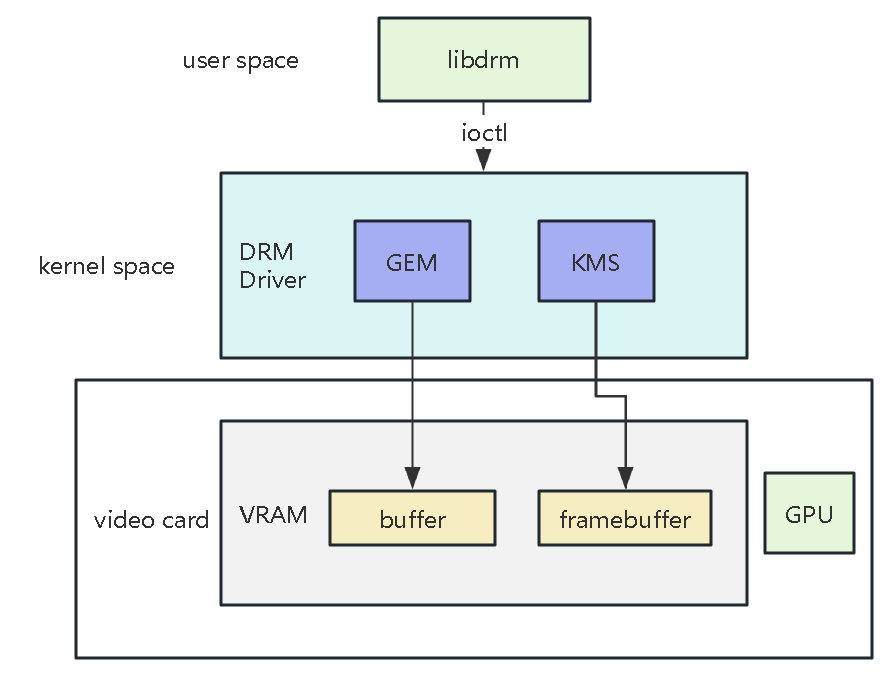
\includegraphics[width=0.6\textwidth]{DRM整体结构.pdf}
  \caption{DRM整体结构}\label{fig:DRM整体结构}
\end{figure}

KMS(Kernel Mode Setting) 内核显示模式设设置,是通过内核来设置和管理显示设备的模式(如分辨率、刷新率、颜色深度等)。
KMS 允许操作系统直接控制显示硬件,减少了用户空间与显示设备之间的中间层,提供了更高效、更灵活的显示控制。显示控制过程如图\ref{fig:DRM显示控制}

GEM(Graphics Execution Manager)是图形缓冲区管理模块,为操作系统和用户空间应用程序提供高效的显存管理功能,实现的功能有缓冲区分配、映射、销毁、交换等,

\begin{figure}[H]
  \centering
  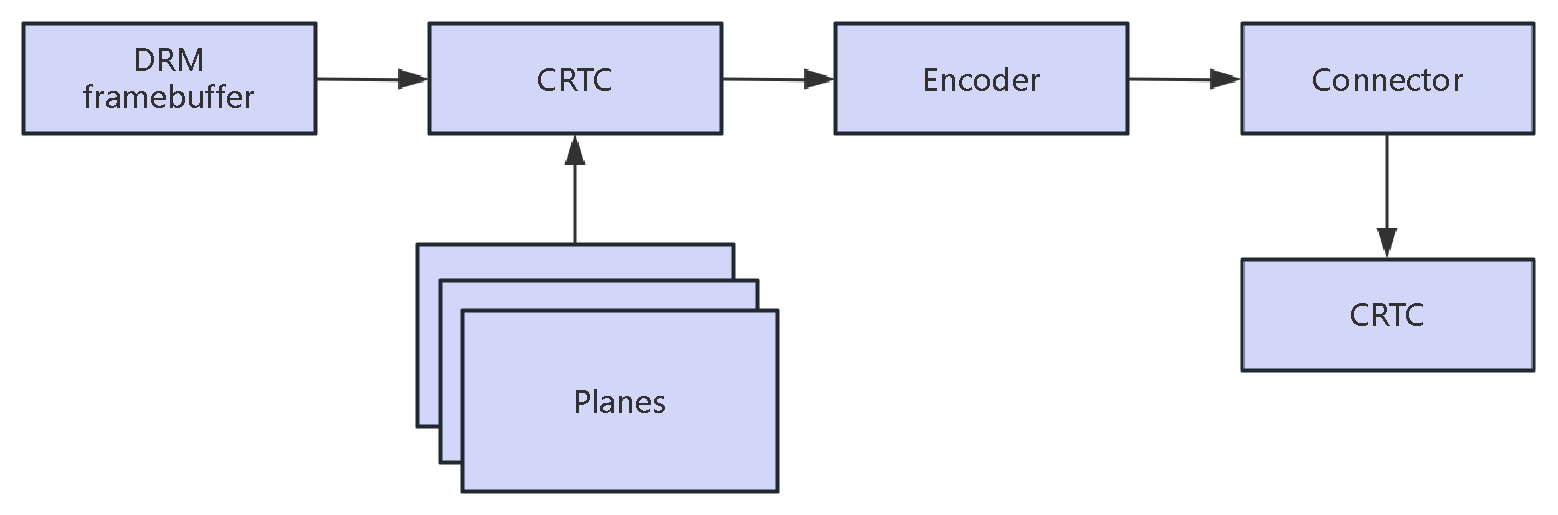
\includegraphics[width=0.8\textwidth]{DRM显示控制.pdf}
  \caption{DRM显示控制}\label{fig:DRM显示控制}
\end{figure}

\section{本章小结}
本章围绕着课题分别介绍了AOSP安卓开源项目、安卓图形系统结构和GPU软件栈等安卓图形相关技术。在AOSP部分,介绍了安卓通用内核、AOSP构建系统与Native程序运行环境、安卓系统架构以及
AOSP源码树4个部分,这些技术是在安卓上实现对龙芯显卡的支持的基础。接着介绍现有的安卓图形协议,分别从低级别组件和高级别组件两部分进行介绍,说明实现对龙芯硬件的支持需要安卓图形系统中的哪些组件。
在最后GPU软件栈中,分别从核模块、MESA、libdrm、DRM4个部分说明除安卓框架外还需要哪些软件实现对硬件的支持。

%dri直接渲染架构还未介绍
